\documentclass[openany]{book}
\usepackage[english]{babel}
\usepackage{biblatex}
\usepackage{amsfonts}
\usepackage{amssymb}
\usepackage{amsmath}
\usepackage{physics}
\newtheorem{problem}{Problem}[chapter]
\usepackage{lipsum}
\usepackage[a4paper, total={6in,8in}]{geometry}
\usepackage{graphicx}
\usepackage{subcaption}
\usepackage{xcolor}
\usepackage{listings}

\definecolor{codegreen}{rgb}{0,0.6,0}
\definecolor{codegray}{rgb}{0.5,0.5,0.5}
\definecolor{backcolour}{rgb}{0.95,0.95,0.92}

\lstdefinestyle{mystyle}{
    backgroundcolor=\color{backcolour},   
    commentstyle=\color{orange},
    keywordstyle=\color{blue},
    numberstyle=\tiny\color{codegray},
    stringstyle=\color{codegreen},
    basicstyle=\ttfamily\footnotesize,
    breakatwhitespace=false,         
    breaklines=true,                 
    captionpos=b,                    
    keepspaces=true,                 
    numbers=left,                    
    numbersep=5pt,                  
    showspaces=false,                
    showstringspaces=false,
    showtabs=false,                  
    tabsize=2
}

\lstset{style=mystyle}

\usepackage{hyperref}

\title{Problems Elementary Mechanical Using Python}
\date{June 16th 2022}

\begin{document}
    \maketitle
    \stepcounter{chapter}
\chapter{First time}
    
    \begin{problem}[Seconds]\label{problem_2.1}
        For this problem we have to
        \begin{enumerate}
            \item Write a script that calculates the number of seconds, $s$, given the number of hours, $h$, according to the formula $s=3600$ $h$
            \item Use the script to find the number of seconds in $1.5$, $12$ and $24$ $h$
        \end{enumerate}
    \end{problem}
    \textit{ Sol. } 
    \lstinputlisting[language=Python]{Programs/chapter2/2_1_seconds.py}
    \begin{verbatim}
        1.5 hours is equivalent 5400.0 seconds
        12.0 hours is equivalent 43200.0 seconds
        24.0 hours is equivalent 86400.0 seconds
    \end{verbatim}


    \begin{problem}[Spherical mass]\label{problem_2.2}
        For this problem we have to
        \begin{enumerate}
            \item Write a script that calculates the mass of a sphere given its radius $r$ and mass density $\rho$ according to the formula $m=\qty(4\pi/3)\rho r^{3}$.
            \item Use the script to find the mass of a sphere of steel of radius $r=1$ mm, $r=1$ m and $r=10$ m.
        \end{enumerate}
    \end{problem}
    \textit{ Sol. }
    \lstinputlisting[language=Python]{Programs/chapter2/2_2_Spherical_mass.py}
    \begin{verbatim}
        The sphere of steel with density 8000 kg/m3
        The sphere with 0.001 m of radius has 3.351032163829113e-05 kg
        The sphere with 1.0 m of radius has 33510.32163829113 kg
        The sphere with 10.0 m of radius has 33510321.638291128 kg
    \end{verbatim}

   
    \begin{problem}[Angle]\label{problem_2.3}
        For this place we have to
        \begin{enumerate}
            \item Write a function that for a point $\qty(x,y)$ returns the angle $\theta$ from the $x$-axis using the formula $\theta = \arctan{\qty(y/x)}$.
            \item Find the angles $\theta$ for the points $\qty(1,1)$, $\qty(-1,1)$, $(-1,-1)$, $(1,-1)$.
            \item How would you change the function to return values of $\theta$ in the range $\qty[0,2\pi]$?
        \end{enumerate}
    \end{problem}


    \begin{problem}[Unit vector]\label{problem_2.4}
        For this problem we have to
        \begin{enumerate}
            \item Write a function that returns the two-dimensional unit vector, $\qty(u_x,u_y)$, corresponding to an angle $\theta$ with the $x$-axis. You can use the formula $\qty(u_x,u_y)=\qty(\cos{\theta},\sin{\theta})$, where $\theta$ is given in radians.
            \item Find the unit vectors for $\theta = 0, \pi/6, \pi/3, \pi/2, 3\pi/2$.
            \item Rewrite the function to instead take the argument $\theta$ in degrees.
        \end{enumerate}
    \end{problem}
    \textit{ Sol. } 
    \lstinputlisting[language=Python]{Programs/chapter2/2_4_Angle.py}
    \begin{verbatim}
The unit vectors for 0 radiants are (1.0, 0.0)
The unit vectors for 0.5235987755982988 radiants are (0.86602540378, 0.49999999999)
The unit vectors for 1.0471975511965976 radiants are (0.50000000000, 0.86602540378)
The unit vectors for 1.5707963267948966 radiants are (6.123233995736766e-17, 1.0)
The unit vectors for 4.71238898038469 radiants are (-1.8369701987210297e-16, -1.0)
    \end{verbatim}


    \begin{problem}[Plotting the normal distribution]\label{problem_2.5}
        The normal distribution, often called the Gaussian distribution, is given as:
        \begin{equation} \label{eqt = normal_distribution}
            P\qty(x;\mu,\sigma) = \frac{1}{\sqrt{2\pi\sigma^{2}}} e^{-\qty(x-\mu)^{2} / \qty(2\sigma)^2}
        \end{equation}
        Where $mu$ is the average and $sigma$ is the standard deviation.
        \begin{enumerate}
            \item Make a function $normal\qty(x,mu,sigma)$ that returns the normal distribution value $P\qty(x,\mu,\sigma)$ as given by the formula \ref{eqt = normal_distribution}.
            \item Use this function to plot the normal distribution for $-5<x<5$ for $\mu=0$ and $\sigma=1$.
            \item Plot the normal distribution for $-5<x<5$ for $\mu=0$ and $\sigma=2$ and $\sigma=0.5$ in the same plot.
            \item Plot the normal distribution $-5<x<5$ for $\sigma=1$ and $\mu=0,1,2$ in three subplots above each other.
        \end{enumerate}
    \end{problem}
    \textit{ Sol. }
    \lstinputlisting[language=Python]{Programs/chapter2/2_5__Plotting_normal.py}
    \begin{figure}[h!]
        \centering
        \begin{subfigure}[b]{0.4\linewidth}
            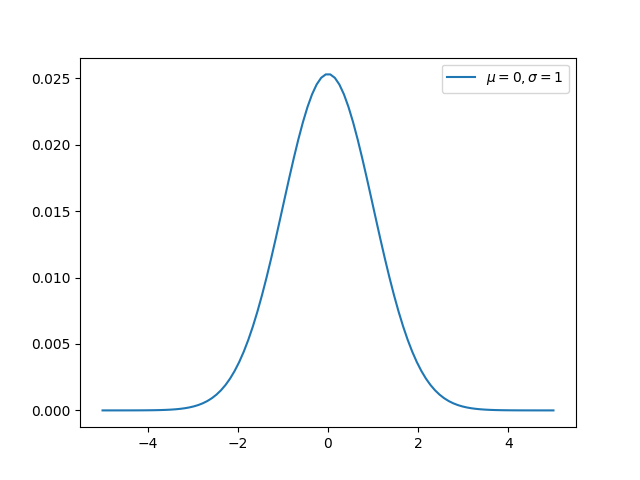
\includegraphics[width=\linewidth]{img/chapter2/2-5/2_5_plot_a.png}
            \caption{For $-5<x<5, \ \mu=0$ and $\sigma=1$}
        \end{subfigure}
        \begin{subfigure}[b]{0.4\linewidth}
            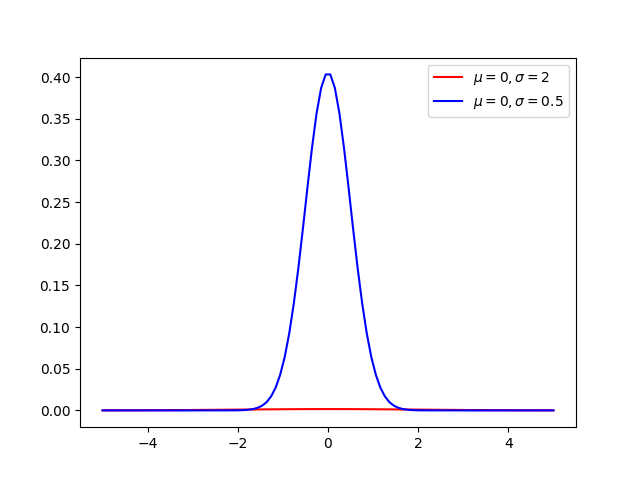
\includegraphics[width=\linewidth]{img/chapter2/2-5/2_5_plot_b.png}
            \caption{For $-5<x<5, \ \mu=0$ and $\sigma=2,0.5$}
        \end{subfigure}
        \begin{subfigure}[b]{0.5\linewidth}
            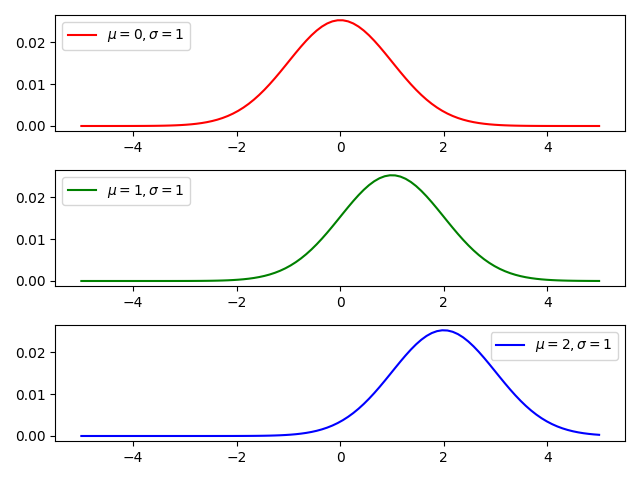
\includegraphics[width=\linewidth]{img/chapter2/2-5/2_5_plot_c.png}
            \caption{For $-5<x<5, \ \mu=0,1,2$ and $\sigma=1$}
        \end{subfigure}
        \caption{Solutions of the problem \ref{problem_2.5}}
        \label{fig:problem 2-5}
    \end{figure}
\end{document}
